% 请确保文件编码为utf-8,使用XeLaTex进行编译,或者通过overleaf进行编译

\documentclass[answers]{exam}  % 使用此行带有作答模块
% \documentclass{exam} % 使用此行只显示题目

\usepackage{xeCJK}
\usepackage{zhnumber}
\usepackage{graphicx}
\usepackage{hyperref}
\usepackage{amsmath}
\usepackage{booktabs}
\usepackage{enumerate}
\usepackage{amssymb}
\usepackage{listings}
\usepackage{floatrow}
\usepackage{blindtext}
\usepackage{subcaption}
\pagestyle{headandfoot}
\firstpageheadrule
\firstpageheader{南京大学}{机器学习导论}{习题四}
\runningheader{南京大学}
{机器学习导论}
{习题四}
\runningheadrule
\firstpagefooter{}{第\thepage\ 页(共\numpages 页)}{}
\runningfooter{}{第\thepage\ 页(共\numpages 页)}{}


\setlength\linefillheight{.5in}

\renewcommand{\solutiontitle}{\noindent\textbf{解:}\par\noindent}

\renewcommand{\thequestion}{\zhnum{question}}
\renewcommand{\questionlabel}{\thequestion .}
\renewcommand{\thepartno}{\arabic{partno}}
\renewcommand{\partlabel}{\thepartno .}

\lstset{language=Matlab}%这条命令可以让LaTeX排版时将Matlab关键字突出显示
\lstset{
	breaklines,%这条命令可以让LaTeX自动将长的代码行换行排版
	basicstyle=\footnotesize\ttfamily, % Standardschrift
	backgroundcolor=\color[rgb]{0.95,0.95,0.95},
	keywordstyle=\color{blue},
	commentstyle=\color{cyan},
	tabsize=4,numbers=left,
	numberstyle=\tiny,
	frame=single,
	%numbers=left, % Ort der Zeilennummern
	numberstyle=\tiny, % Stil der Zeilennummern
	%stepnumber=2, % Abstand zwischen den Zeilennummern
	numbersep=5pt, % Abstand der Nummern zum Text
	tabsize=2, % Groesse von Tabs
	extendedchars=false, %
	breaklines=true, % Zeilen werden Umgebrochen
	keywordstyle=\color{red},%这一条命令可以解决代码跨页时, 章节标题, 页眉等汉字不显示的问题
	stringstyle=\color{white}\ttfamily, % Farbe der String
	showspaces=false, % Leerzeichen anzeigen ?
	showtabs=false, % Tabs anzeigen ?
	xleftmargin=17pt,
	framexleftmargin=17pt,
	framexrightmargin=5pt,
	framexbottommargin=4pt,
	%backgroundcolor=\color{lightgray},
	showstringspaces=false % Leerzeichen in Strings anzeigen ?
}
\renewcommand{\lstlistingname}{CODE}
\lstloadlanguages{% Check Dokumentation for further languages ...
	%[Visual]Basic
	%Pascal
	%C
	Python
	%XML
	%HTML
	%Java
}
%%% load AMS-Latex Package
\usepackage{amssymb}
\usepackage{amsmath,amsfonts}
% \usepackage{amsthm}
\usepackage{amsopn}
\usepackage{bm} % bold symbol
\usepackage{multirow}



% operator in optimization
\DeclareMathOperator{\argmax}{arg\,max}
\DeclareMathOperator{\argmin}{arg\,min}
\DeclareMathOperator{\softmax}{softmax}

% special functions
\newcommand{\trace}[1]{\operatornamewithlimits{tr}\left\{#1\right\}}
\newcommand{\diag}{\operatornamewithlimits{diag}}
\newcommand{\sign}{\operatornamewithlimits{sign}}
\newcommand{\const}{\operatornamewithlimits{const}}

% special display
\newcommand{\parde}[2]{\frac{\partial #1}{\partial  #2}}

% define vector and matrix symbols
\newcommand{\vct}[1]{\boldsymbol{#1}} % vector
\newcommand{\mat}[1]{\boldsymbol{#1}} % matrix
\newcommand{\cst}[1]{\mathsf{#1}}  % constant

% shorthand
\newcommand{\vtheta}{\vct{\theta}}
\newcommand{\vmu}{\vct{\mu}}
\newcommand{\vc}{\vct{c}}
\newcommand{\vp}{\vct{p}}
\newcommand{\vq}{\vct{q}}
\newcommand{\vx}{{\vct{x}}}
\newcommand{\vy}{\vct{y}}
\newcommand{\vz}{{\vct{z}}}
\newcommand{\vu}{\vct{u}}
\newcommand{\vo}{{\vct{o}}}
\newcommand{\va}{\vct{a}}
\newcommand{\vb}{\vct{b}}
\newcommand{\ve}{\vct{e}}
\newcommand{\vr}{\vct{r}}
\newcommand{\vt}{\vct{t}}
%\newcommand{\vpsi}{\vct{\psi}}
\newcommand{\vs}{\vct{s}}
\newcommand{\vv}{\vct{v}}
\newcommand{\vw}{\vct{w}}
\newcommand{\vzero}{\vct{0}}
\newcommand{\vf}{\vct{f}}
\newcommand{\vh}{\vct{h}}
\newcommand{\vg}{\vct{g}}
\newcommand{\vphi}{\vct{\phi}}
\newcommand{\vpsi}{\vct{\psi}}
\newcommand{\ones}{\vct{1}}
\newcommand{\mU}{\mat{U}}
\newcommand{\mA}{\mat{A}}
\newcommand{\mB}{\mat{B}}
\newcommand{\mC}{\mat{C}}
\newcommand{\mD}{\mat{D}}
\newcommand{\mV}{\mat{V}}
\newcommand{\mW}{\mat{W}}
\newcommand{\mH}{\mat{H}}
\newcommand{\mI}{\mat{I}}
\newcommand{\mP}{\mat{P}}
\newcommand{\mS}{\mat{S}}
\newcommand{\mJ}{\mat{J}}
\newcommand{\mM}{\mat{M}}
\newcommand{\mT}{\mat{T}}
\newcommand{\mZ}{\mat{Z}}
\newcommand{\mO}{\mat{O}}
\newcommand{\mX}{\mat{X}}
\newcommand{\mY}{\mat{Y}}
\newcommand{\mQ}{\mat{Q}}
\newcommand{\mLambda}{\mat{\Lambda}}
% \newcommand{\mL}{\mat{L}}
\newcommand{\mmI}{\mat{I}}
\newcommand{\mK}{\mat{K}}
\newcommand{\mSigma}{\mat{\Sigma}}
\newcommand{\mOmega}{\mat{\Omega}}
\newcommand{\cC}{\cst{C}}
\newcommand{\cM}{\cst{M}}
\newcommand{\cN}{\cst{N}}
\newcommand{\cQ}{\cst{Q}}
\newcommand{\cD}{\cst{D}}
\newcommand{\cL}{\cst{L}}
\newcommand{\cK}{\cst{K}}
\newcommand{\cH}{\cst{H}}
\newcommand{\cR}{\cst{R}}
\newcommand{\cU}{\cst{U}}
\newcommand{\cS}{\cst{S}}
\newcommand{\cX}{\cst{X}}
\newcommand{\sQ}{\mathcal{Q}}
\newcommand{\sS}{\mathcal{S}}
\newcommand{\sF}{\mathcal{F}}
\newcommand{\sC}{\mathcal{C}}
\newcommand{\sX}{\mathcal{X}}
\newcommand{\sH}{\mathcal{H}}

\newcommand{\bE}{\mathbb{E}}
\newcommand{\bR}{\mathbb{R}}
\newcommand{\bH}{\mathbb{H}}

\usepackage{algorithm}  
% \usepackage{algorithmic}
%\usepackage{algorithmicx}  
\usepackage{algpseudocode}  

\floatname{algorithm}{算法}  
\renewcommand{\algorithmicrequire}{\textbf{输入:}}  
\renewcommand{\algorithmicensure}{\textbf{输出:}}  

\begin{document}
\Large
\noindent
% 姓名学号
姓名:麻超 \\
学号:201300066 \\
\begin{questions}
    \question [20] \textbf{神经网络基础} \\

    给定训练集$D=\{(\vx_1, \vy_1), (\vx_2, \vy_2), ..., (\vx_m, \vy_m)\}$. 其中$\vx_i \in \bR^d$,
    $\vy_i \in \bR^l$表示输入示例由$d$个属性描述,
    输出$l$维实值向量.
    图~\ref{ch5_img:mlp}给出了一个有$d$个输入神经元、$l$个输出神经元、$q$个隐层神经元的多层神经网络, 其中输出层第$j$个神经元的阈值用$\theta_j$表示, 隐层第$h$个神经元的阈值用$\gamma_h$表示. 输入层第$i$个神经元与隐层第$h$个神经元之间的连接权为$v_{ih}$,
    隐层第$h$个神经元与输出层第$j$个神经元之间的连接权为$w_{hj}$.
    记隐层第$h$个神经元接收到的输入为$\alpha_h=\sum_{i=1}^d v_{ih}x_i$,
    输出层第$j$个神经元接收到的输入为$\beta_j=\sum_{h=1}^q w_{hj}b_h$,
    其中$b_h$为隐层第$h$个神经元的输出.
    \begin{figure}[ht]
        \centering
        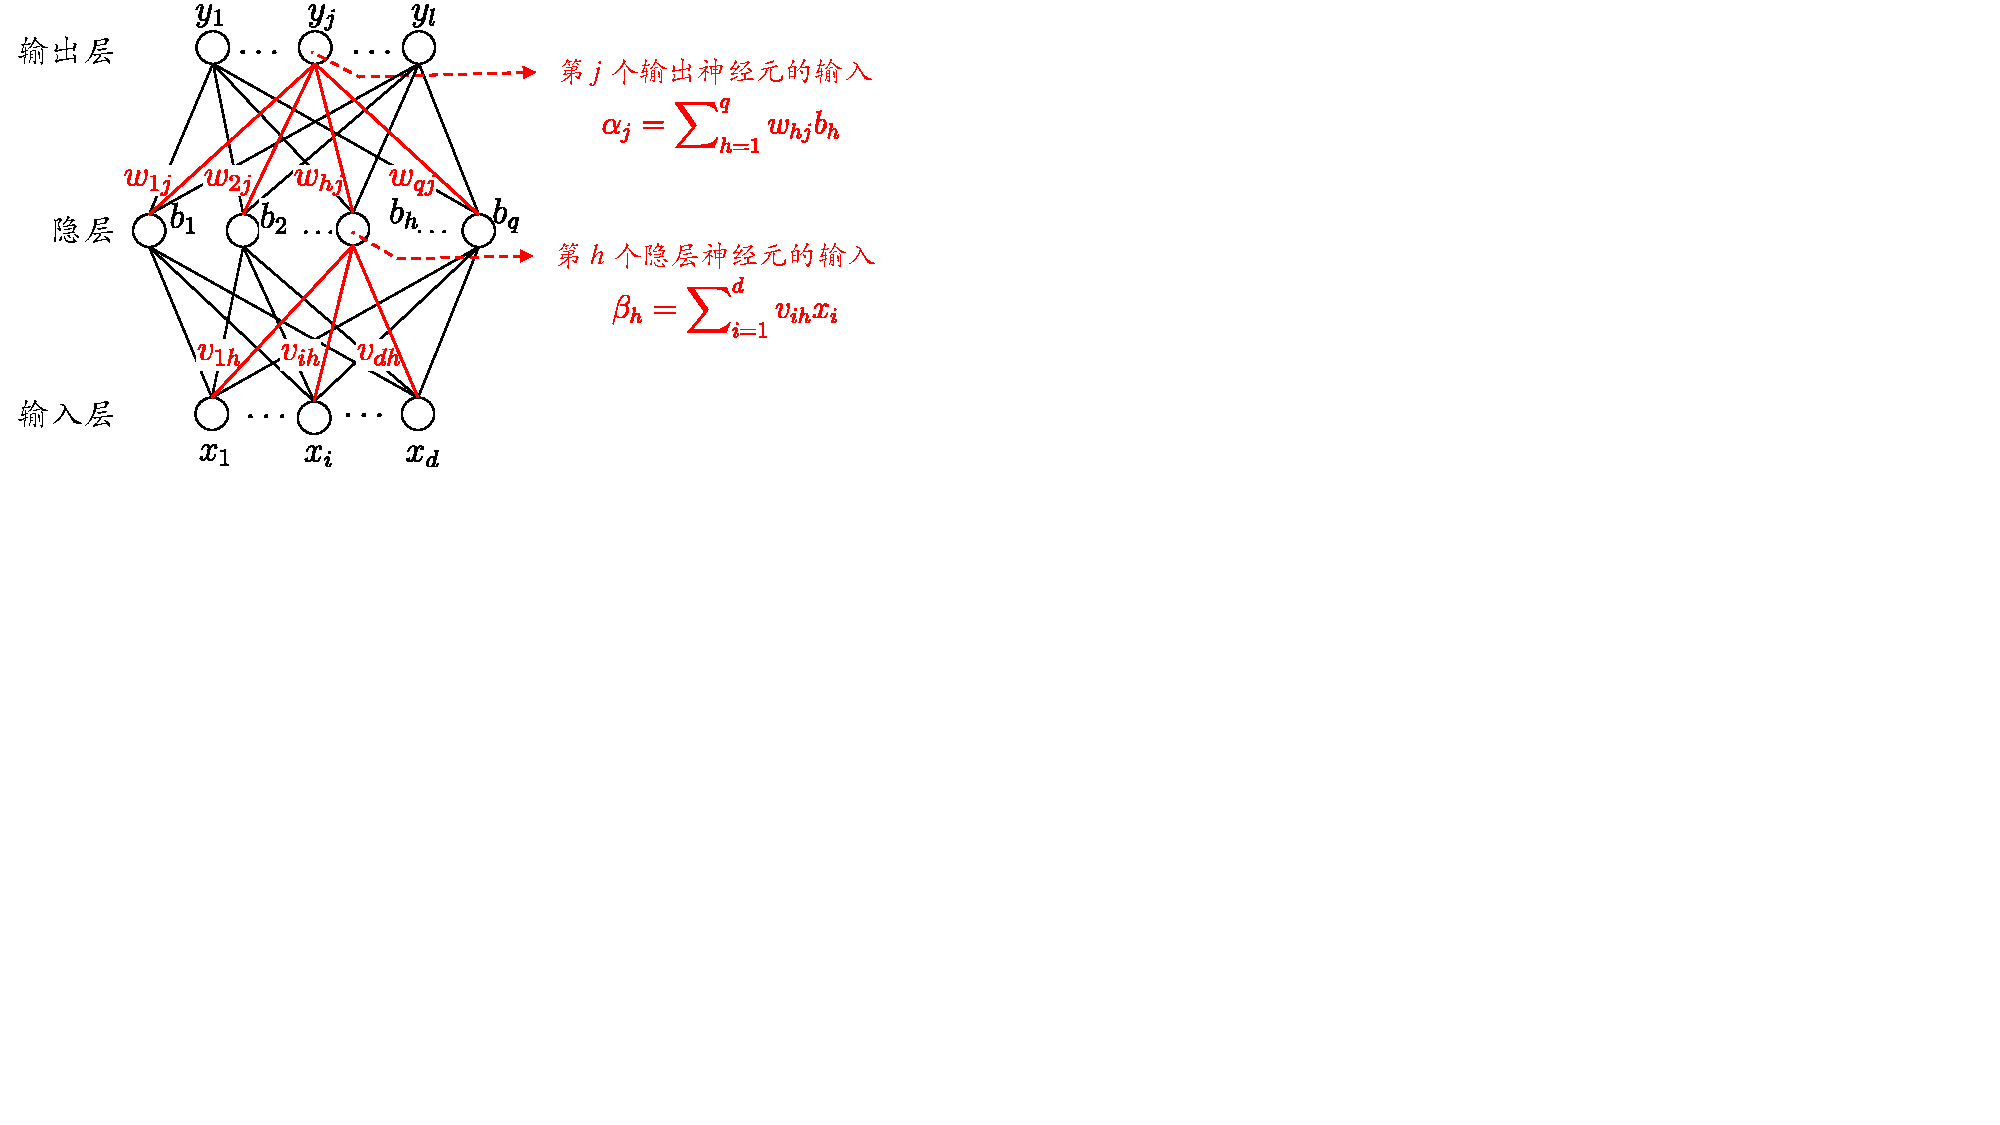
\includegraphics[width=0.70\textwidth]{figure/ch5_nn.pdf}
        \caption{多层神经网络(教材图5.7)}\label{ch5_img:mlp}
    \end{figure}

    不同任务中神经网络的输出层往往使用不同的激活函数和损失函数,
    本题介绍几种常见的激活和损失函数, 并对其梯度进行推导.
    \begin{enumerate}
        \item 在二分类问题中($l=1$), 标记$y\in\{0,1\}$, 一般使用Sigmoid函数作为激活函数,
              使输出值在$[0, 1]$范围内, 使模型预测结果可直接作为概率输出.
              Sigmoid函数的输出一般配合二元交叉熵 (Binary Cross-Entropy) 损失函数使用,
              对于一个训练样本$(\vx, y)$有
              \begin{equation}
                  \ell(y, \hat{y}_1) = - \left[ y \log(\hat{y}_1) + (1 - y) \log(1 - \hat{y}_1) \right]
              \end{equation}
              %   请计算$\frac{\partial \ell(y, \hat{y}_1)}{\partial \beta_j}$, 
              %   并写出其向量形式, 即$\frac{\partial \ell(y, \hat{y}_1)}{\partial \vct{\beta}}$.
              记$\hat{y}_1$为模型对样本属于正类的预测结果, 请计算$\frac{\partial \ell(y, \hat{y}_1)}{\partial \beta_1}$,
        \item 当$l>1$, 网络的预测结果为$\hat{\vy}\in\mathbb{R}^l$, 其中$\hat{y}_i$表示输入被预测为第$i$类的概率. 对于第$i$类的样本, 其标记$\vy\in\{0,1\}^l$, 有$y_i=1$,
              $y_j=0, j \neq i$. 对于一个训练样本$(\vx, \vy)$, 交叉熵损失函数$\ell(\vy, \hat{\vy})$的定义如下
              \begin{equation}
                  \ell(\vy, \hat{\vy}) = - \sum_{j = 1}^{l} y_j \log \hat{y}_j
              \end{equation}
              在多分类问题中, 一般使用Softmax层作为输出, Softmax层的计算公式如下
              \begin{equation}
                  \hat{y}_j = \frac{e^{{\beta}_j}}{\sum_{k=1}^{l} e^{\vct{\beta}_k}}
              \end{equation}\label{ch5_ep:softmax}
              易见Softmax函数输出的$\hat{\vy}$
              符合$\sum_{j=1}^{l} \hat{y}_j = 1$,
              所以可以直接作为每个类别的概率. Softmax输出一般配合交叉熵(Cross Entropy)
              损失函数使用, 请计算$\frac{\partial \ell(\vy, \hat{\vy})}{\partial \beta_j}$,
              %   并写出其向量形式, 即$\frac{\partial \ell(\vy, \hat{\vy})}{\partial \vct{\beta}}$.
              %   请计算$\frac{\partial \ell(\vy, \hat{\vy})}{\partial \vct{\beta}}$.
        \item 分析在二分类中使用Softmax和Sigmoid的联系与区别.
        \item KL散度 (Kullback-Leibler divergence) 定义了两个分布之间的距离, 对于两个离散分布$Q(x)$和$P(x)$, 其定义为
              \begin{equation}
                  D_{\operatorname{KL}}(P\;\|\;Q) = \sum_{x \in \mathcal{X}} P(x)\log \left(\frac{P(x)}{Q(x)} \right)
              \end{equation}
              其中$\mathcal{X}$为$x$的取值空间. 试分析交叉熵损失函数和KL散度的关系.

    \end{enumerate}


    \begin{solution}
        \begin{enumerate}
            \item 根据已知条件,有:
                  \begin{align*}
                      f'(\beta_1,\theta_1)                                 & =f(\beta_1,\theta_1)\cdot (1-f(\beta_1,\theta_1))                                                        \\
                      \frac{\partial \ell (y,\hat{y}_1)}{\partial \beta_1} & =\frac{\partial \ell (y,\hat{y}_1)}{\partial \hat{y}_1}\cdot \frac{\partial \hat{y}_1}{\partial \beta_1} \\
                                                                           & =(-\frac{y}{\hat{y}_1}+\frac{1-y}{1-\hat{y}_1})\cdot \hat{y}_1\cdot (1-\hat{y}_1)                        \\
                                                                           & =-y+\hat{y}_1
                  \end{align*}
            \item
                  \begin{align*}
                      \frac{\partial \ell (\vy,\hat{\vy})}{\partial \beta_j} & = \frac{\partial \ell (\vy,\hat{\vy})}{\partial \hat{\vy}_j}\cdot \frac{\hat{\vy}_j}{\partial \beta_j}+\sum_{k=1,j\neq k}^{l}\frac{\partial \ell (\vy,\hat{\vy})}{\partial \hat{\vy}_k} \cdot \frac{\partial \ell (\hat{\vy}_k)}{\partial \beta_j} \\
                                                                             & =-\vy_j(1-\hat{\vy}_j)+\sum_{k=1,j\neq k}^l \vy_k(1-\frac{\sum_{m=1,m\neq j}^{l}e^\beta m}{e^\beta k}\cdot \hat{\vy}_k )
                  \end{align*}
            \item 联系:在二分类问题中,Sigmoid与Softmax输出结构相同,均为$\frac{1}{1+e^{x_2-x_1}} $.
                  区别:它们在二分类问题的输出原理不同.其中Sigmoid针对于两点式分布问题,结果中,可以分为该类的概率为P,则不能分到该类的概率为1-P.与之对应,Softmax方法针对多分类问题,在化简至二分类时仍保留其思想,其正例和反例概率分别计算.
            \item 交叉熵是熵与KL散度的和.\\
                  在计算损失的过程中,二者等价.
                  \begin{align*}
                      D_{KL}(P||Q) & =\sum_{x\in \mathcal{X}}P(x)\log(\frac{P(x)}{Q(x)} )                       \\
                                   & =\sum_{x\in \mathcal{X}}P(x)(\log P(x)-\log Q(x) )                         \\
                                   & =\sum_{x\in \mathcal{X}}P(x)\log P(x)-\sum_{x\in \mathcal{X}}P(x)\log Q(x) \\
                                   & =-S(P)+\ell (P,Q)
                  \end{align*}
                  其中$S$为熵,当$S(A)$为常数时,最小化KL散度等同于最小化交叉熵.
        \end{enumerate}
    \end{solution}

    \question [20] \textbf{运算的向量化} \\
    在编程实践中, 一般需要将运算写成向量或者矩阵运算的形式, 这叫做运算的向量化 (vectorization).
    向量化可以充分利用计算机体系结构对矩阵运算的支持加速计算,
    大部分数学运算库例如\lstinline{numpy}也对矩阵计算有专门的优化.
    另一方面, 如果一个运算可以写成向量计算的形式, 会更容易写出其导数形式并进行优化.
    本题中举两个简单的例子
    \begin{enumerate}
        \item 给定示例矩阵$\mX \in \bR^{m\times d}$, 表示$m$个示例(向量), 每个示例有$d$维,
              计算$m$个示例两两之间的距离矩阵$\mD \in \bR^{m\times m}$,
              两个向量之间的欧式距离定义为$\|\vx - \vy\|_2=\sqrt{\sum_{i=1}^{d} (x_i - y_i)^2}$.
              求距离矩阵可以通过循环的方式, 即\lstinline{plain_distance_function}中实现的方法;
              \lstinputlisting[language=Python]{code/ch5/vectorization_plain_distance.py}
        \item 输入一个矩阵$\mX \in \bR^{m\times d}$, 表示$m$个向量, 每个向量有$d$维,
              要求对输入矩阵的行按照一个给定的排列$\vct{p}=\{p_{1}, p_{2}, ..., p_m\}$进行重新排列.
              即输出一个新的矩阵$\mX^\prime$, 其中第$i$行的内容为输入矩阵的第$p_{i}$行.
              假设重排列为一个函数$\operatorname{perm}$即$\mX^\prime = \operatorname{perm}(\mX)$, 已知梯度$\frac{\partial \ell}{\partial \mX^\prime}$,
              需要计算$\frac{\partial \ell}{\partial \mX}$. 对矩阵的行进行排列可以采用简单的循环实现, 例如\lstinline{plain_permutation_function}中的实现方法.
              \lstinputlisting[language=Python]{code/ch5/vectorization_plain_permutation.py}
    \end{enumerate}
    请给出上述两种任务的向量化实现方案,并分析上述实现方法和向量化实现方法之间运行时间的差异。(提示:比如可以针对不同规模的矩阵大小来尝试分析主要操作的运行时间)

    \begin{solution}
        %请在此处作答
    \end{solution}


    \question [20] \textbf{支持向量机}

    考虑标准的SVM优化问题如下(即教材公式(6.35)),
    \begin{equation}
        \begin{aligned}
            \min _{\vw, b, \xi_{i}} \quad & \frac{1}{2}\|\vw\|^{2}+C \sum_{i=1}^{m} \xi_{i}     \\
            \text { s.t. } \quad          & y_{i}\left(\vw^\top \vx_{i}+b\right) \geq 1-\xi_{i} \\
                                          & \xi_{i} \geq 0, i\in [m] .
        \end{aligned}
    \end{equation}
    注意到, 在(2.1)中, 对于正例和负例, 其在目标函数中分类错误的“惩罚”是相同的. 在实际场景中, 很多时候正例和负例错分的“惩罚”代价是不同的(参考教材2.3.4节). 比如考虑癌症诊断问题, 将一个确实患有癌症的人误分类为健康人, 以及将健康人误分类为患有癌症, 产生的错误影响以及代价不应该认为是等同的. 所以对负例分类错误的样本(即false positive)施加$k>0$倍于正例中被分错的样本的“惩罚”. 对于此类场景下
    \begin{enumerate}
        \item 请给出相应的SVM优化问题.
        \item 请给出相应的对偶问题, 要求详细的推导步骤, 如KKT条件等.
    \end{enumerate}

    \begin{solution}
        \begin{enumerate}
            \item
                  \begin{align*}
                      \min _{\vw, b, \xi_{i}} \quad & \frac{1}{2}\|\vw\|^{2}+C \sum_{i=1}^{m} s_i\xi_{i}  \\
                      \text { s.t. } \quad          & y_{i}\left(\vw^\top \vx_{i}+b\right) \geq 1-\xi_{i} \\
                                                    & \xi_{i} \geq 0, i\in [m] .
                  \end{align*}
                  其中,$s_i$为第$i$个训练样本对C的加权系数,负例分类错误时为k,正例分类错误时为1.
            \item 令$\alpha,\mu$表示拉格朗日乘子,有:
                  \begin{align*}
                      L(\vw,b,\xi,\alpha,\mu)                     & =\frac{1}{2} \|\vw\|^{2}+C\sum_{i=1}^{m}s_i\xi_i                           \\
                                                                  & +\sum_{i=1}^{m}\alpha_i(1-\xi_i-y_i(\vw \vx_i+b))-\sum_{i=1}^{m}\mu_i\xi_i \\
                      \because \Delta_{\vw}L                      & =\Delta_{b}L=\Delta_{\xi_i}L=0                                             \\
                      \therefore w-\sum_{i=1}^{m}\alpha_iy_i\vx_i & =\sum_{i=1}^{m}\alpha_iy_i=Cs_i-(\alpha_i+\mu_i)=0
                  \end{align*}
                  故对偶问题为:
                  \begin{align*}
                      \max _{\alpha} \quad & \sum_{i=1}^{m}\alpha_i-\frac{1}{2} \sum_{i=1}^{m}\sum_{j=1}^{m}(\alpha_i\alpha_jy_iy_j\vx_i^T\vx_j) \\
                      \text { s.t. } \quad & \sum_{i=1}^{m}y_i\alpha_i=0                                                                         \\
                                           & 0\leq \alpha_i\leq s_iC ,i\in [m].
                  \end{align*}
                  KKT条件为:
                  $$
                      \begin{cases}
                           & y_i(\vw^T\vx_i+b)-1+\xi_i\geq 0                                 \\
                           & \alpha_i(y_i(\vw^T\vx_i+b)-1+\xi_i\geq 0)=0,\mu_i\xi_i=0        \\
                           & \alpha_i,\mu_i,\xi_i\geq 0                                      \\
                           & \vw=\sum_{i=1}^{m}\alpha_iy_i\vx_i,\sum_{i=1}^{m}\alpha_i,y_i=0
                      \end{cases}
                  $$
        \end{enumerate}
    \end{solution}
    \question [20] \textbf{核函数} \\
    教材6.3节介绍了Mercer定理, 说明对于一个二元函数 $k(\cdot, \cdot)$, 当且仅当对任意 $m$ 和 $\{\vx_{1}, \vx_{2}, \ldots, \vx_{m}\}$, 它对应的Gram矩阵(核矩阵)是半正定的时, 它是一个有效的核函数. 核矩阵 $\mK$ 中的元素为 $K_{i j}=\kappa\left(\vx_{i}, \vx_{j}\right)$. 请根据Mercer定理证明以下核函数是有效的.

    \begin{enumerate}
        \item $\kappa_{3}=a_{1} \kappa_{1}+a_{2} \kappa_{2}$, 其中 $a_{1}, a_{2} \geq 0$.
        \item $f(\cdot)$ 是任意实值函数, 由 $\kappa_{4}\left(\vx, \vx^{\prime}\right)=f(\vx) f\left(\vx^{\prime}\right)$ 定义的 $\kappa_{4}$.
        \item 由 $\kappa_{5}\left(\vx, \vx^{\prime}\right)=\kappa_{1}\left(\vx, \vx^{\prime}\right) \kappa_{2}\left(\vx, \vx^{\prime}\right)$ 定义的 $\kappa_{5}$.
        \item 由 $\kappa_{6}\left(\vx, \vx^{\prime}\right)=f(\vx) \kappa_{1}\left(\vx, \vx^{\prime}\right)f(\vx')$定义的 $\kappa_{6}$
    \end{enumerate}
    \begin{solution}
        \begin{enumerate}
            \item 对于任意非零向量$x$,有:
                  \begin{align*}
                      x^TK_3x & =x^T(a_1K_1+a_2K_2)x           \\
                              & =a_1x^TK_1x+a_2x^TK_2x         \\
                      \because a_1,a_2>0,x^TK_1x,x^TK_2x\geq 0 \\
                      \therefore x^TK_3x\geq 0
                  \end{align*}
                  因此$K_3$半正定,故核函数有效.
            \item 定义对称矩阵$M$如下:
                  $$
                      M=diag(f(x),f(x),...,f(x))
                  $$
                  其对应的核函数可以看作两个矩阵的乘积,即$K_4=MM^T$.故$K_4$为半正定矩阵,$k_4$为核函数.
            \item 只需证明两个半正定矩阵的直积仍然是半正定矩阵,可以定义$K_5=K_1\circ K_2$.
                  \begin{align*}
                      y^TK_5y & =y^T(K_1\circ K_2)y                                                  \\
                              & =\sum_{i=1}^{m}\sum_{j=1}^{m}k_1(x_i,x_j)k_2(x_i,x_j)y_iy_j          \\
                              & =tr(diag(y_1,y_2,...,y_m)K_1 diag(y_1,y_2,...,y_m)K_2^T)             \\
                              & =tr(diag(y_1,y_2,...,y_m)AA^T diag(y_1,y_2,...,y_m)BB^T)             \\
                              & =tr(B \quad diag(y_1,y_2,...,y_m)A(B\quad diag(y_1,y_2,...,y_m)A)^T) \\
                              & =tr(PP^T)\geq 0
                  \end{align*}
                  所以$k_5$是一个核函数.
            \item $K_1$为半正定矩阵,可以将其写成$K_1=NN^T$.故$k_6$的核矩阵为:
                  $$
                      K_6=MNN^TM^T=MN(MN^T).
                  $$
                  这是一个半正定矩阵,故$k_6$是一个核函数.
        \end{enumerate}
    \end{solution}

    \question [20] \textbf{主成成分分析} \\
    $\vx \in \bR^{d}$ 是一个随机向量, 其均值和协方差分别是 $\vmu=\mathbb{E}(\vx) \in \bR^{d}$, $\mSigma=\mathbb{E}(\vx-\vmu_\vx)(\vx-\vmu_\vx)^{\top} \in \bR^{d \times  d}$. 定义随机变量 $\{y_{i}=\vu_{i}^{\top} \vx+a_{i} \in \bR, i=1, \ldots, {d'} \leq d\}$ 为 $\vx$ 的主成分, 其中 $\vu_{i} \in \bR^{d}$ 是单位向量($\vu_i^\top \vu_i = 1$), $a_{i} \in \bR$, $\left\{y_{i}\right\}_{i=1}^{{d'}}$ 是互不相关的零均值随机变量, 它们的方差满足 $\operatorname{var}\left(y_{1}\right) \geq \operatorname{var}\left(y_{2}\right) \geq \cdots \geq \operatorname{var}\left(y_{{d'}}\right)$. 假设 $\mSigma$ 没有重复的特征值.
    \begin{enumerate}
        \item  请证明$\{a_{i}=-\vu_{i}^{\top} \vmu\}_{i=1}^{d'}$.
        \item 请证明$\vu_{1}$ 是 $\mSigma$ 最大的特征值对应的特征向量. (提示: 写出要最大化的目标函数, 写出约束条件, 使用拉格朗日乘子法)
        \item 请证明$\vu_{2}^{\top} \vu_{1}=0$,且 $\vu_{2}$ 是 $\mSigma$ 第二大特征值对应的特征向量. (提示: 由 $\left\{y_{i}\right\}_{i=1}^{d}$ 是互不相关的零均值随机变量可推出 $\vu_{2}^{\top} \vu_{1}=0$, 可作为第二小问的约束条件之一)
        \item 通过PCA进行降维, 得到的随机变量满足$\operatorname{var}\left(y_{1}\right) \geq \operatorname{var}\left(y_{2}\right) \geq \cdots \geq \operatorname{var}\left(y_{d}\right)$, 也就是降维后的数据 在不同维度上有不同的方差, 从而导致不同维度的数值范围差异很大, 如果想要降维后的样本在不同维度具有大致相同的数值范围, 应该怎么做?
    \end{enumerate}
    \begin{solution}
        \begin{enumerate}
            \item 由于$\{y_i\}_{i=1}^{d'}$为互不相关的零均值随机变量,所以有:
                  \begin{align*}
                      \mathbb{E}(y_i)=\mathbb{E}(\vu_i^T)=0
                  \end{align*}
                  所以可以得到:
                  \begin{align*}
                       & \vu_i^T\mathbb{E}(x)+a_i=0 \\
                       & a_i=-\vu                   \\\vu_i^T\mathbb{E}(x)
                  \end{align*}
            \item
                  由于需要最大化主成分的方差,所以可以得到如下的优化目标:
                  $$
                      \max \quad \sum_{i=1}^{d'}var(y_i)
                  $$
                  又
                  \begin{align*}
                      var(y_i) & =\mathbb{E}(y_i^2)-\mathbb{E}(y_i)^2                                                              \\
                               & =\mathbb{E}(y_i^2)                                                                                \\
                               & =\mathbb{E}(\vu_i^T\vx\cdot\vu_i^T\vx+2(-\vu_i^T\mu\cdot \vu_i^T\vx)+\vu_i^T\mu\cdot \mu \vu_i^T) \\
                               & =\mathbb{E}(\vu_i^T(x-\mu)(x-\mu)^T\vu_i)                                                         \\
                               & =\vu_i^T\sum \vu_i
                  \end{align*}
                  所以原目标可以写为如下形式:
                  \begin{align*}
                      \min  \quad          & -\sum_{i=1}^{d'}\vu_i^T\sum \vu_i \\
                      \text { s.t. } \quad & \vu_i^T\vu_i=1,i\in[m]            \\
                  \end{align*}
                  该问题的Lagrange函数为:$$
                      L(\vu_i,v_i)=-\sum_{i=1}^{d'}u_i^T\sum \vu_i+\sum_{i=1}^{d'}v_i(\vu_i^T\vu_i-1)
                  $$
                  其Lagrange乘子为$v_i\geq 0$.分别求偏导得到:
                  \begin{align*}
                       & \frac{\partial L}{\partial \vu_i}=-2\sum \vu_i+2v_i\vu_i=0 \\
                       & \frac{\partial L}{\partial v_i}=\vu_i^T\vu_i-1=0
                  \end{align*}
                  所以有$\sum \vu_i=v_i\vu_i$.故$v_i$是协方差矩阵$\sum$对应的特征值,$\vu_i$是协方差矩阵$\sum$的特征向量,且:
                  $$
                      var(y_i)=\vu_i^T\sum \vu_i=v_i\vu_i^T\vu_i=v_i
                  $$
                  故$var(y_i)$对应的向量$\vu_i$就是最大特征值$v_i$对应的特征向量.
            \item 由题意可以得到新的优化问题,即:
                  \begin{align*}
                      \max _{\vu_i\in\{\vu_i\}_{i=1}^{d'}} \quad & \vu_i^T(\vx-\mu)(x-\mu)^T\vu_i                \\
                      \text { s.t. } \quad                       & \vu_i^T\vu_i=1,\vu_i\in \{\vu_i\}_{i=1}^{d'}  \\
                                                                 & \vu_i^T\vu_i=0,\vu_i\in \{\vu_i\}_{i=2}^{d'}.
                  \end{align*}
                  其Lagrange函数为:
                  $$
                      L(\vu_i,\lambda_i,\beta_i)=\vu_i^T(\vx-\mu)(\vx-\mu)^T\vu_i-\lambda_i(\vu_i^T\vu_i-1)-\beta_i\vu_i^T\vu_1
                  $$
                  分别求偏导可得:
                  \begin{align*}
                      \frac{\partial L}{\partial \vu_i}     & =2(\vx-\mu)(\vx-\mu)^T\vu_i-2\lambda_i\vu_i-\beta_i\vu_1=0 \\
                      \frac{\partial L}{\partial \lambda_i} & =\vu_i^T\vu_i-1=0                                          \\
                      \frac{\partial L}{\partial \beta_i}   & =\vu_i^T\vu_1=0
                  \end{align*}
                  于是有:
                  \begin{align*}
                      \vu_i^T(\vx-\mu)(\vx-\mu)^T\vu_i-\vu_i^T\frac{1}{2} \beta_i\vu_1=\vu_1^T\lambda_i\vu_i=\lambda_i\vu_i^T\vu_i=0 \\
                      \vu_i^T\sum_x \vu_i=\frac{1}{2} \beta_i
                  \end{align*}
                  由于$\sum_x$为对称矩阵,可以得到
                  $$
                      \frac{1}{2} \beta_i=\vu_i^T\sum_x\vu_1=\vu_i^T\lambda_1\vu_1=0
                  $$
                  所以可以得到$\beta=0$.\\
                  此时就与上一问几乎一直,即最大化$\lambda_i$,且$\lambda_2$为最大,故$\vu_2$是$\sum$第二大的特征值对应的特征向量.
            \item 可以在PCA降维前对数据进行标准化处理,也就是对数据先减去均值再除以标准差,此时就可以使得均值为0,标准差为1.
        \end{enumerate}
    \end{solution}
\end{questions}


\end{document}